\section{Ordered densities of squared singular values of a Gaussian matrix product}

%%%%%%%%%%%%%%%%%%%%%%%%%%%%%%%%%%%%%%%%%%%%%%%%%%%%%%%%%%%%%%%%%%%%%%%%%%%%%%%%
% 015 Math macros
\newcommand{\G}[7]{\mathrm{G}^{\tiny\begin{bmatrix}
			#1&#2\\#3&#4
	\end{bmatrix}}\left(\begin{matrix}
		#5 \\ #6
	\end{matrix}\;\middle|\;#7\right)}
%%%%%%%%%%%%%%%%%%%%%%%%%%%%%%%%%%%%%%%%%%%%%%%%%%%%%%%%%%%%%%%%%%%%%%%%%%%%%%%%

\emph{This rather simple result is a humble acknowledgment of the great work in finite-size random matrix theory (RMT) by Prof. Gernot Akemann and team at Uni Bielefeld. For finding the ordered densities, a straightforward recursive formulation, in terms of the \href{https://mathworld.wolfram.com/MeijerG-Function.html}{$\mathrm{MeijerG}$ function}, based on the work of Alberto Zanella at CNR in Italy, is utilized.}

Note: Several integration formulas for the MeijerG function are known, e.g., see the \href{https://mathworld.wolfram.com/MeijerG-Function.html}{$\mathrm{MeijerG}$ function reference}. Although the expressions are complex, they can be numerically evaluated quite easily via Mathematica or MATLAB. It amazes me that these finite-size RMT densities are even analytically approachable, although, undoubtedly, the asymptotic RMT theory is ``more elegant.''

The theorem is as follows. See below for Mathematica code and numerical simulations.

\begin{theorem}
	\label{thm:qk}
	Let $\boldsymbol{X}$ and $\boldsymbol{Y}$ be independent $m\times l$ and $l\times q$ random matrices, respectively, $q \leq m \leq l,$ with identical and independently distributed elements $[\boldsymbol{X}]_{ij}, \sim \mathcal{CN}(0,1), i=1,\dots,m,j=1,\dots,l,$ and $[\boldsymbol{Y}]_{ij}, \sim \mathcal{CN}(0,1), i=1,\dots,l,j=1,\dots,q,$ respectively. Let $x_1 \geq \dots \geq x_q$ denote the squared singular values of the product $\boldsymbol{X}\boldsymbol{Y}.$ The pdf of the $k$-th squared singular value of $\boldsymbol{X}\boldsymbol{Y},$ denoted by $q_k(x_k; m, l, q),$ is given by
	\begin{align}
		q_k(x_k; m, q) = K_{q_k} h^{[k,(),()]}_k(x_k; m, l, q),
	\end{align}
	where $K_{q_k}$ is a constant ensuring that the integral over the pdf is equal to one, and function $h^{[d,\boldsymbol{n},\boldsymbol{m}]}_k(x_k; m, q)$ is given by the recurrence relation
	\begin{align}
		\sum_{i = 1}^{|{\mathcal{I}}^{[d,\boldsymbol{n}]}|} \sum_{j = 1}^{|{\mathcal{I}}^{[d,\boldsymbol{m}]}|} h^{[d-1,\boldsymbol{n}',\boldsymbol{m}']}_k(x_k; m,l,q), \label{eqn:qkrec}
	\end{align}
	$[l,(),()]$ denotes the initial value of $[d,\boldsymbol{n},\boldsymbol{m}],$ and ``()'' denotes the empty tuple. Tuples $\boldsymbol{n}$ and $\boldsymbol{m}$ are updated as $\boldsymbol{n}' \coloneqq \boldsymbol{n} \cup \{(i,[{\mathcal{I}}^{[d,\boldsymbol{n}]}]_i)\}$ and $\boldsymbol{m}' \coloneqq \boldsymbol{m} \cup \{(j,[{\mathcal{I}}^{[d,\boldsymbol{m}]}]_j)\},$ where $i$ and $j$ are the summation indices in (\ref{eqn:qkrec}), and $[{\mathcal{I}}^{[d,\boldsymbol{n}]}]_i$ and $[{\mathcal{I}}^{[d,\boldsymbol{m}]}]_j$ are the $i$-th and $j$-th elements of sets ${\mathcal{I}}^{[d, \boldsymbol{n}]}$ and ${\mathcal{I}}^{[d, \boldsymbol{m}]},$ respectively, defined as ${\mathcal{I}}^{[d,\boldsymbol{n}]} \coloneqq \{1,2,\dots,q\} \setminus \pi_2(\boldsymbol{n})$ and ${\mathcal{I}}^{[d,\boldsymbol{m}]} \coloneqq \{1,2,\dots,q\} \setminus \pi_2(\boldsymbol{m}).$ Next, the termination step is given below
		\begin{align}
			h^{[1,\boldsymbol{n},\boldsymbol{m}]}_k(x_k; m, q) &= \sum_{i = 1}^{|{\mathcal{I}}^{[d,\boldsymbol{n}]}|} \sum_{j = 1}^{|{\mathcal{I}}^{[d,\boldsymbol{m}]}|} s\left(\boldsymbol{n}',\boldsymbol{m}'\right)
			\G{2}{0}{0}{2}{-}{v_2+n-1, m+n+v_1-2}{x_k} \nonumber\\
			&\qquad \times \det{\boldsymbol{\Xi}\left(k, m, q, {\mathcal{I}}^{[d+1,\boldsymbol{n}']},{\mathcal{I}}^{[d+1,\boldsymbol{m}']}\right)} \nonumber\\
			&\qquad \times \prod_{p = 1}^{k-1} \G{3}{0}{1}{3}{1}{0, v_2+[{\mathcal{I}}^{[d,\boldsymbol{n}]}]_p, [{\mathcal{I}}^{[d,\boldsymbol{m}]}]_p + [{\mathcal{I}}^{[d,\boldsymbol{n}]}]_p+v_1 - 1}{x_k}\label{eqn:qkf2term}
		\end{align}
	where $v_1=l-q, v_2=m-q,$ $G$ is the Meijer G function \cite{Olver2010}, $\boldsymbol{\Xi}\left(k, m, q, {\mathcal{I}}^{[d+1,\boldsymbol{n}']},{\mathcal{I}}^{[d+1,\boldsymbol{m}']}\right)$ is a $(q-l)\times (q-l)$ matrix with elements 
	\begin{equation}
		\left[\G{2}{1}{1}{3}{1}{v_2+n,m+n+v_1-1,0}{x_k}\right]_{ij}, \label{eqn:qkf2mat}
	\end{equation}
	and $i,j=1,\dots,q-l,$
	\begin{align}
		s\left(\boldsymbol{n}',\boldsymbol{m}'\right) &= (-1)^{\sum_{i=1}^{|\boldsymbol{n}'|} [\pi_1(\boldsymbol{n}')]_i + [\pi_1(\boldsymbol{m}')]_i},
	\end{align}
	and $\gamma(\cdot,\cdot)$ denotes the lower incomplete Gamma function.
\end{theorem}

Second projection notation: Let set $s := \{(1,2), (3,4), (5,6)\}$ be a set containing three tuples. Then, $\pi_2(s)$ is the second projection of $s$ given by $\pi_2(s) = \{2, 4, 6\}.$ Below, a sketch of the proof for completeness.

\begin{proof}
	The joint pdf of the squares of the singular values of $\boldsymbol{X}\boldsymbol{Y}$ is given in \cite[(18)]{Akemann2013},\cite{Ipsen2015} as
	\begin{align}
		K_q \prod_{1\leq i < j \leq q} (x_j-x_i) \det{\boldsymbol{\Delta}},
	\end{align}
	where $\boldsymbol{\Delta}$ is a $q \times q$ matrix with elements
	\begin{equation}
		\left[\G{2}{0}{0}{2}{-}{v2,v1+j-1}{x_i}\right]_{ij},
	\end{equation}
	with $i,j=1,\dots,q.$ The pdf of the $k$-th eigenvalue can be obtained via the procedure given in \cite[Sec. IV-B]{Zanella2009} utilizing the function
	\begin{equation}
		\varphi(n,m,x) = \G{2}{0}{0}{2}{-}{v_2+n-1, m+n+v_1-2}{x},
	\end{equation}
	and the integrals in \cite[(A7)]{Akemann2013} and \cite{Olver2010} to integrate over the Meijer G function. Lastly, the multiple summations in \cite[Sec. IV-B]{Zanella2009} can be equivalently reformulated to obtain the recursive definition given in (\ref{eqn:qkrec}) and (\ref{eqn:qkf2term}).
\end{proof}

\subsection{Mathematica Reference Code}

Now, a Mathematica package for evaluating the ordered densities is as follows. Here, in \verb!xyz[symb_, l, v_2, v_1, q_]!, $symb$ is the desired symbol for the variable, e.g., $x, l$ is the index (corresponding to $k$ in the theorem), $v_1, v_2,$ and $q$ are as in the theorem above.

\begin{lstlisting}[language=Mathematica,numbers=none]
(* ::Package:: *)

BeginPackage["xyl`"]
(*** Exported Symbol ***)
xyl
Begin["`Private`"]

\[CurlyPhi][v2_, v1_, q_, n_, m_] := MeijerG[{{}, {}}, {{v2+n-1, m + n+v1 - 2}, {}}, s]; 
Iup[v2_, v1_, q_, n_, m_] := MeijerG[{{}, {1}}, {{0, v2+n, m + n+v1 - 1}, {}}, s]; 
Idown[v2_, v1_, q_, n_, m_] := MeijerG[{{1}, {}}, {{v2+n, m + n+v1 -1}, {0}}, s]; 
r[i_, n_, q_] := Complement[Range[q], n][[i]]
sg[n_, m_, q_] := Product[(-1)^(FirstPosition[Complement[Range[q], m[[1 ;; i - 1]]], m[[i]]] + FirstPosition[Complement[Range[q], n[[1 ;; i - 1]]], n[[i]]]), {i, 1, Length[n]}]
Dmat[l_, v2_, v1_, q_, ns_, ms_] := Piecewise[{{1, l == q}}, Det[Table[Idown[v2, v1, q, r[n, ns, q], r[m, ms, q]], {n, 1, q - l}, {m, 1, q - l}]]]
xylpdf[l_, v2_, v1_, q_, d_, ns_, ms_] := Sum[xylpdf[l, v2, v1, q, d - 1, Append[ns, n], Append[ms, m]], {n, Complement[Range[q], ns]}, {m, Complement[Range[q], ms]}]
xylpdf[l_, v2_, v1_, q_] := xylpdf[l, v2, v1, q, l, {}, {}]
xylpdf[l_, v2_, v1_, q_, 1, ns_, ms_] := Product[Iup[v2, v1, q, ns[[i]], ms[[i]]], {i, 1, l - 1}]*
Sum[\[CurlyPhi][v2, v1, q, n, m]*sg[Append[ns, n], Append[ms, m], q]*Dmat[l, v2, v1, q, Append[ns, n], Append[ms, m]], {n, Complement[Range[q], ns]}, {m, Complement[Range[q], ms]}]
xyl[symb_,l_?NumericQ,v2_?NumericQ,v1_?NumericQ,q_?NumericQ] := xylpdf[l, v2, v1, q]/(Product[Gamma[n] Gamma[n+v1] Gamma[n+v2],{n,1,q}] Factorial[l-1]) /. s->symb ;

End []
EndPackage[]
\end{lstlisting}

\subsection{Numerical Results}

Lastly, the numerical simulations for $v_1 = 6, v_2 = 2,$ and $q = 2.$ We see that the results based on the above expressions and those based on Monte-Carlo simulations agree well.

\begin{figure}[H]
	\centering
	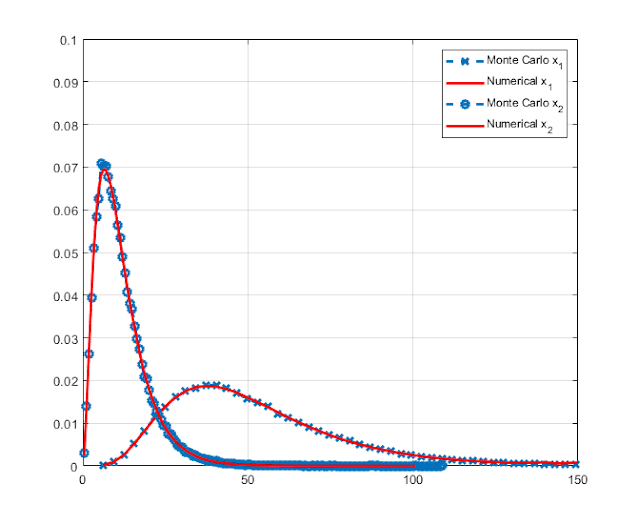
\includegraphics[width=0.95\textwidth,keepaspectratio]{015_004_1.png}
\end{figure}

- ARK

\subsection{Version History}
\begin{enumerate}
	\item \emph{First published: 9th Jul. 2022 on aravindhk-math.blogspot.com}
	\item \emph{Edited: 16th Dec. 2023 -- converted theorem and proof images to \LaTeX}
\end{enumerate}


